%Präambel:
\documentclass{scrartcl}						% Vor dem Drucken auf scrartcl ändern
\usepackage[ngerman]{babel}
\usepackage[utf8]{inputenc}					% für Sonderzeichen
\usepackage[T1]{fontenc}					% zur Umsetzung von Sondereichen
\usepackage{url}
\usepackage[pdfborder ={0 0 0}]{hyperref}	% für Verlinkungen
\usepackage{enumitem}						% Zum Nummerieren
\usepackage{amsmath}						% Math. Zeichen
\usepackage{amssymb}						% Math. Symbole
\usepackage{graphicx}						% Bilder einfügen
\usepackage{longtable}						% Tabellen über eine Seite
\usepackage{subfigure}						% Zwei Bilder nebeneinander
\usepackage{wrapfig}
\usepackage{caption}						% Hilfsmittel, damit Bilder nicht auf die nächste Seite geschoben werden
\usepackage[decimalsymbol=comma]{siunitx}				% Für schöne Einheiten mit Komma
            


\title{Lock-In-Verstärker}
\author{Friedrich Möller und Wilhelm Eschen}

\begin{document}
	\maketitle
	\tableofcontents
	\clearpage
			

\section{Aufgaben}

	
\clearpage

\section{Grundlagen}
		
		
	\clearpage
				 
\section{Auswertung}		
		\subsection{Versuchstag 1 - Grundlagen des Lock-In Verstärkers}
			In Aufgabe 1.1 untersuchten wir die einzelnen Bestandteile eines Lock-In-Verstärkers. Begonnen haben wir hierbei in Aufgabe 1.1.a mit dem Breitbandverstärker. Es ergab sich die folgende Amplitudenübertragungsfunktion, bei einer Generatorspannung von $ 10 \ mV_{pp} $.
			
			\begin{figure}[h!]
				\centering
				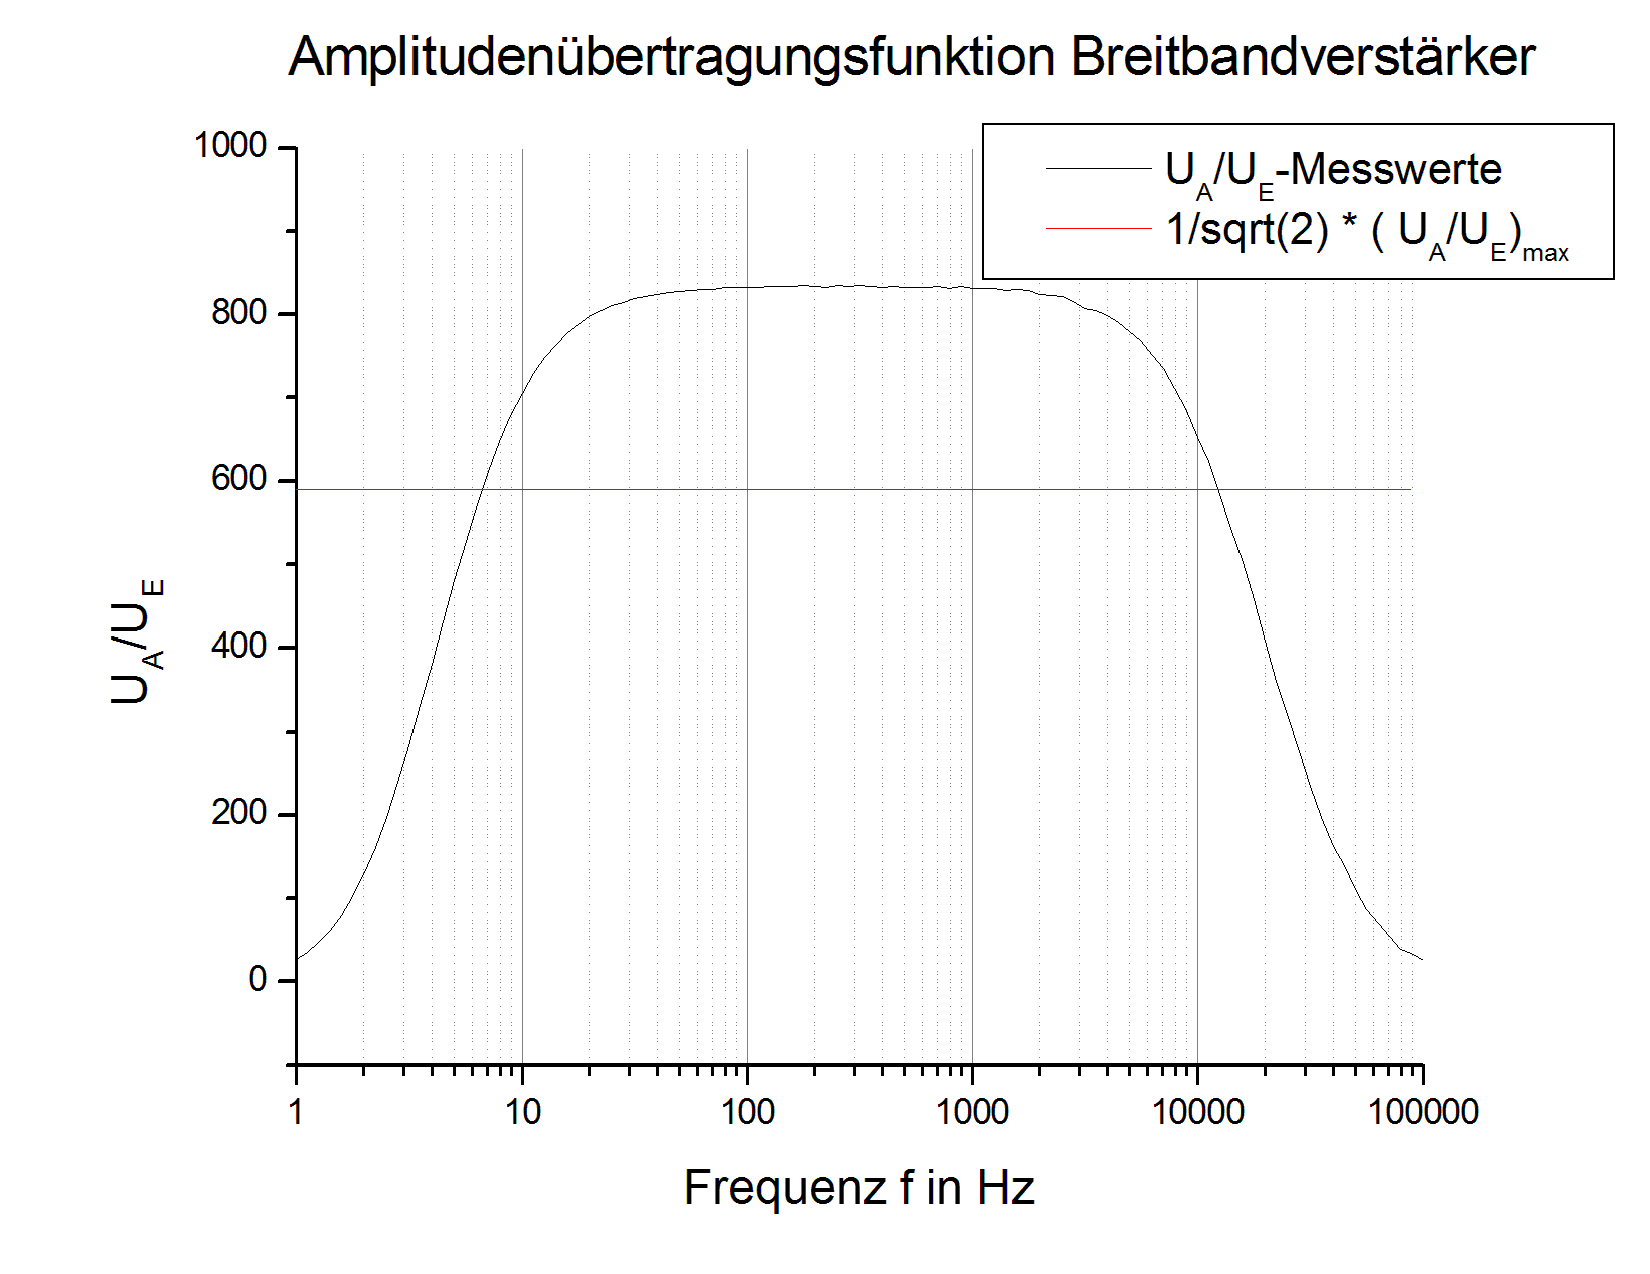
\includegraphics[scale=0.4]{A1a}
				\caption{Amplitudenübertragungsfunktion Breitbandverstärker}
			\end{figure}
			In das Diagramm ist zusätzlich eine Gerade eingezeichnet, welche den $ \frac{U_{max}}{\sqrt{2}} $ anzeigt. Die Schnittpunkte dieser Geraden mit der Amplitudenübertragungsfunktion ergeben die obere und untere Grenzfrequenz $ f_{unten} $ und $ f_{oben} $. Die Differenz beider liefert uns die gesuchte Bandbreite unseres Breitbandverstärkers.
			\begin{equation*}
				\Delta f=f_{oben}-f_{unten}=11500 \ Hz - 7 \ Hz = 11493 \ Hz
			\end{equation*}
			\newline
			Als nächstes sollten die beiden TT-Filter für 25Hz und 180Hz untersucht werden. Auch dazu wurden die Amplitudenübertragungsfunktionen aufgenommen. Daraus lassen sich analog die obere und untere Grenzfrequenz ablesen, sowie die Bandbreite berechnen. Die Güte der Filter ergibt sich nach $ Q=\frac{f_{Grenz}}{\Delta f} $. Der 25Hz-TT-Filter wurde mit einer Spannungsamplitude von $10 \ mV_{pp}$ und der 180Hz-TT-Filter mit $1\ V_{pp}$ gemessen. Es ergaben sich die folgenden Verläufe.
			\clearpage
			\begin{figure}[h!]
					\centering
					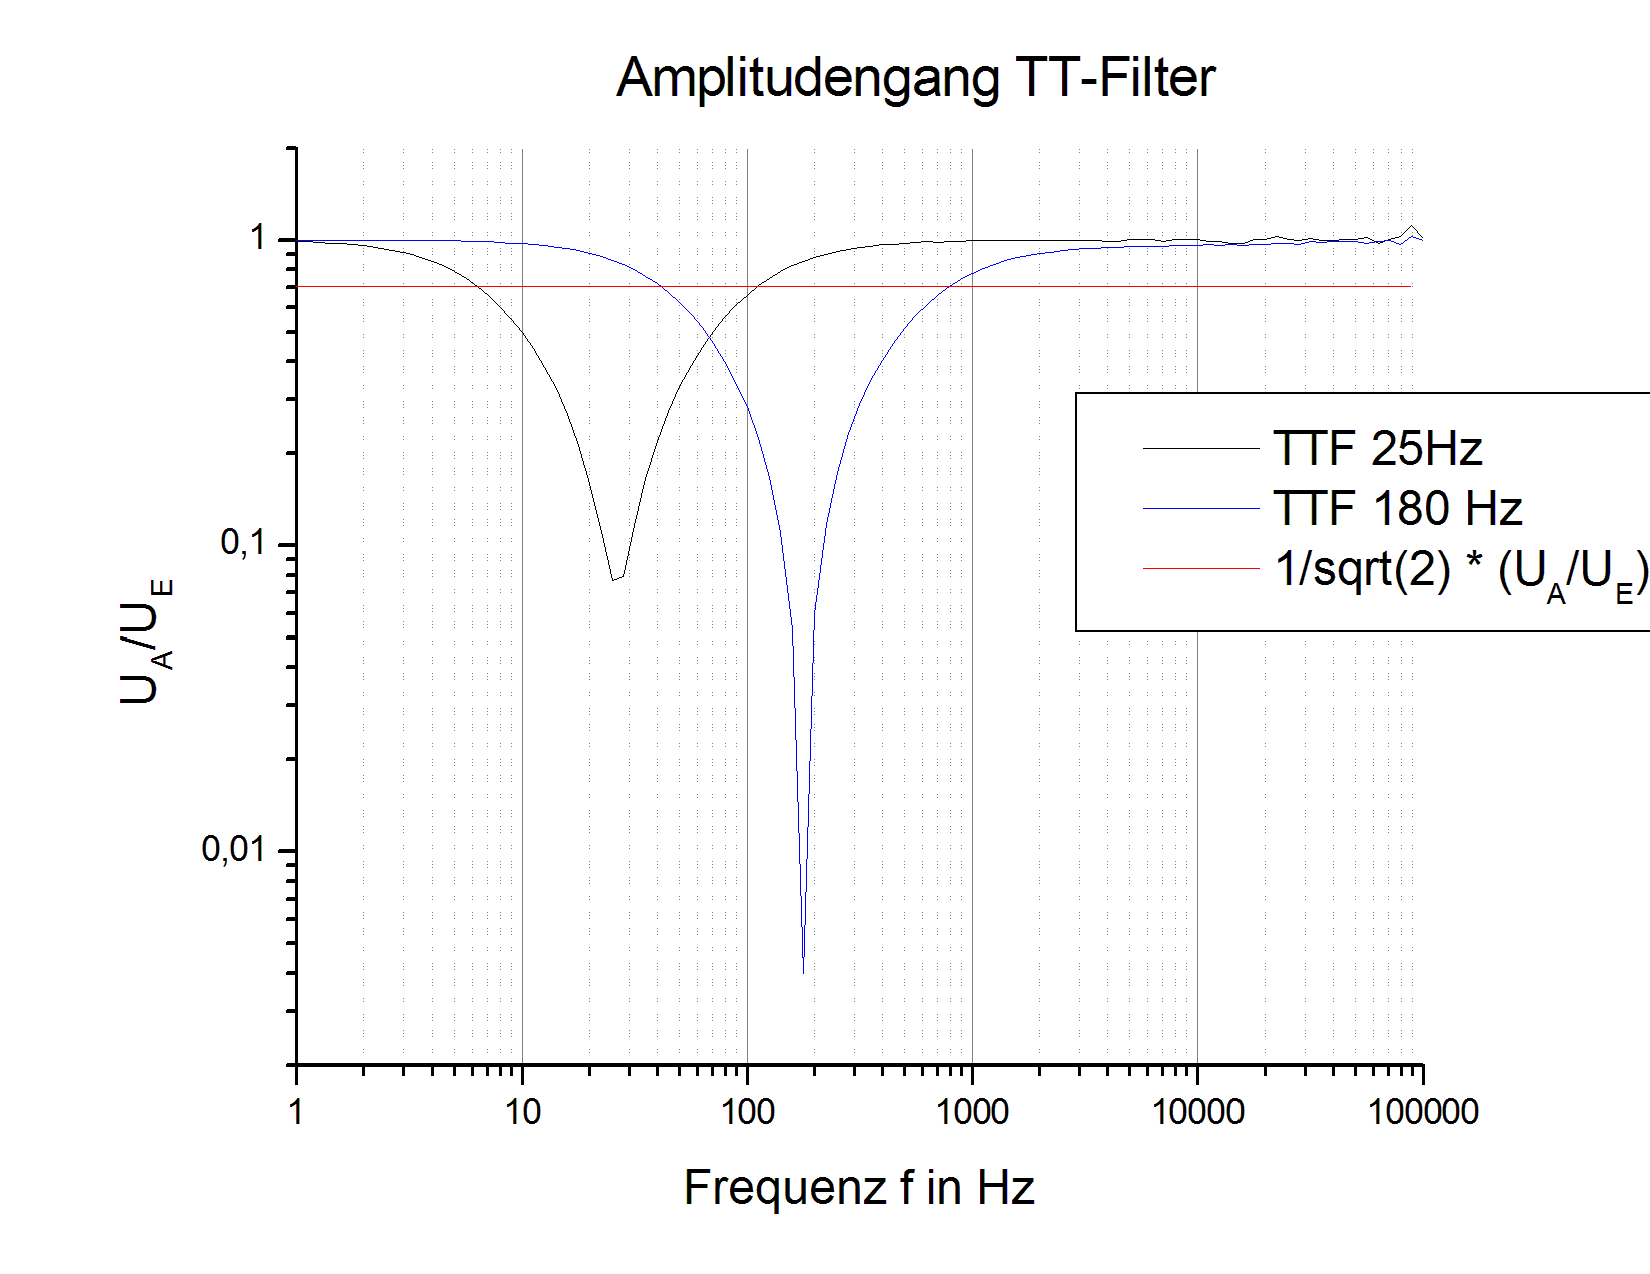
\includegraphics[scale=0.4]{A1b}
					\caption{Amplitudenübertragungsfunktion TT-Filter}
			\end{figure}
			
			In der Tabelle sind alle Werte zusammengefasst:
			\center
			\begin{tabular}{|c|c|c|c|c|}
			\hline $f_{grenz} $ in Hz & $f_{unten}$ in Hz & $f_{oben}$ in Hz & $\Delta f$ in Hz & Güte Q \\ 
			\hline 25 & 6,2 & 110 & 103,8 & 0,241 \\ 
			\hline 180 & 41 & 800 & 759 & 0,237 \\ 
			\hline 
			\end{tabular} 
			\flushleft
			
			Anschließend haben wir  in Aufgabe 1.1.c den TT-Filter für 180Hz in die Rückkopplung des Bandbreitenverstärkers eingefügt. Für den dadurch entstandenen Schmalbandverstärker haben wir für drei Rückkopplungsgrade von 3,5 und 7 (=Stellradeinstellung) den Amplitudengang aufgenommen. Daraus kann man abermals die Grenzfrequenzen, die Bandbreite und die Güte bestimmen. Die Daten sind in der folgenden Tabelle zusammengefasst.
			\center
			\begin{tabular}{|c|c|c|c|c|c|}
			\hline Rückkopplungsgrad & $f_{grenz}$ in Hz & $f_{unten}$ in Hz & $f_{oben}$ in Hz & $\Delta f$ in Hz & Güte Q \\ 
			\hline 3 & 230 & 130 & 426 & 296 & 0,777 \\ 
			\hline 5 & 210 & 130 & 300 & 170 & 1,240 \\ 
			\hline 7 & 200 & 130 & 240 & 110 & 1,818 \\ 
			\hline 
			\end{tabular}
			\flushleft Die Werte liesen sich aus dem nachfolgendem Diagramm ablesen. Die Ablesefehler werden hierbei vernachlässigt.
			\begin{figure}[h!]
					\centering
					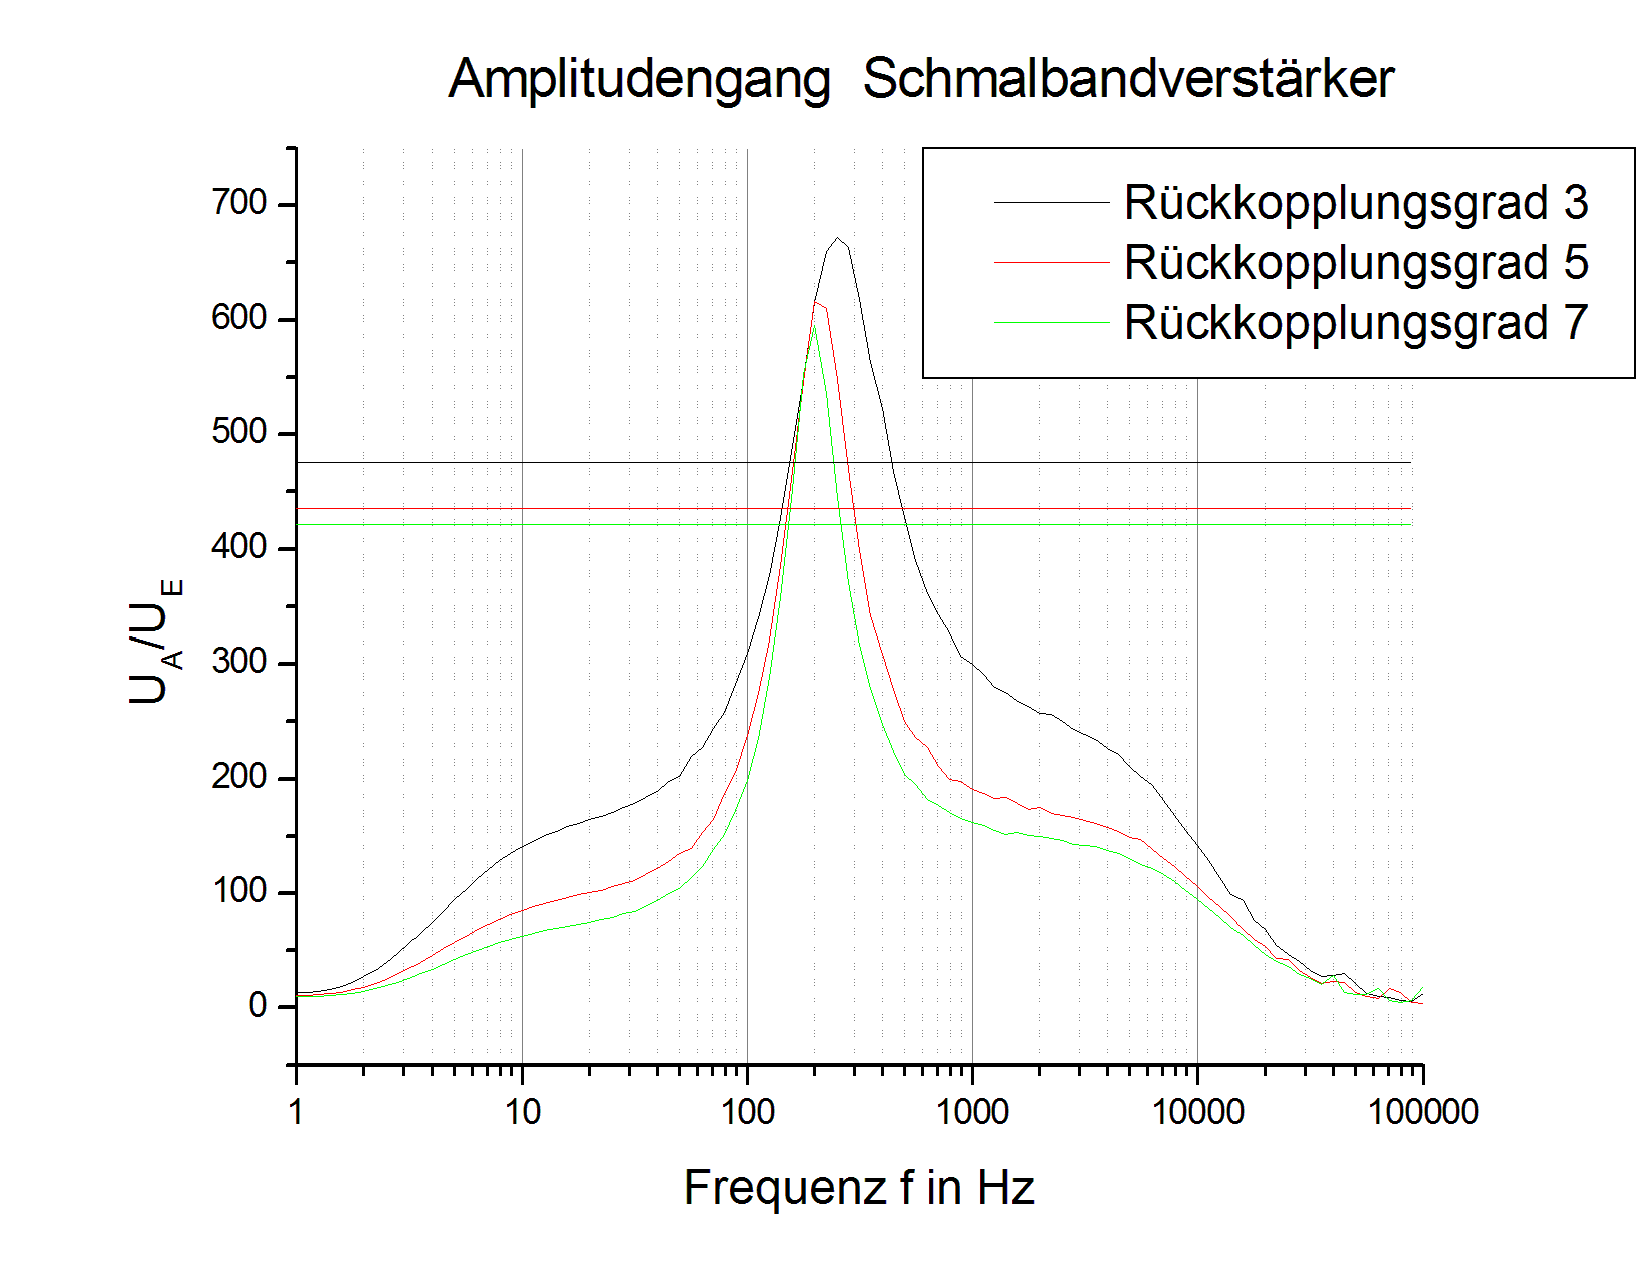
\includegraphics[scale=0.4]{A1c}
					\caption{Amplitudengang Schmalbandverstärker für versch. Rückkopplungsgrade}
			\end{figure}
			
			Mit steigendem Rückkopplungsgrad steigt auch die Güte des Schmalbandverstärkers. Im Vergleich zu dem Breitbandverstärker hat sich die Güte mehr als verdreifacht (von 0,24 auf 0,78 bei dem geringsten vermessenen Rückkopplungsgrad).\\
			
			Um in Aufgabe 1.1.d die maximale Phasenverschiebung zu bestimmen, welche mit dem vorliegenden Phasenschieber bei 180Hz Referenzsignal zu erreichen ist, haben wir das Referenzsignal an das Oszilloskop auf Kanal 1 und den Ausgang des Phasenempfindlichen Gleichrichters (PEG), der mit 5V und 0V gespeist wurde, auf Kanal 2 gelegt. Im DUAL-Modus konnten nun zwischen den beiden Signalen die zeitliche Verschiebung gemessen werden, welche sich gemäß 
			\begin{equation*}
				\frac{\Delta t}{T}=\frac{\Delta \phi}{360^\circ} \ \ \ \ \Rightarrow \ \ \ \ \Delta \phi=f\cdot \Delta t \cdot 360^\circ
			\end{equation*}
			in eine Phasenverschiebung umrechnen lässt. Es wurden folgende Werte gemessen.
			\center
			\begin{tabular}{|c|c|c|c|}
			\hline U in V & Stellrad Phase & $\Delta t$ in ms & $ \Delta \phi$ in $^\circ$ \\ 
			\hline 0 & 8 & 2,96 & 191,8 \\ 
			\hline 0 & 13 & 0,41 & 26,6 \\ 
			\hline 5 & 8 & 0,19 & 12,3 \\ 
			\hline 5 & 13 & 2,45 & 158,8 \\ 
			\hline 
			\end{tabular} 
			\flushleft
			Folglich lässt sich für 0V am PEG und ein Referenzsignal von f=180Hz eine maximale Phasenverschiebung von $ 191,8^\circ $ und für 5V eine von $ 158,8^\circ $ einstellen.\\
			
			In Aufgabe 1.1.e sollte nun die Gleichrichtungswirkung des PEG untersucht werden. Dafür nahmen wir Bilder bei Einwegegleichrichtung und Zweiwegegleichrichtung auf.
			\clearpage
			Zunächst für die Einwegegleichrichtung:
			
			\begin{figure}[h!]
				\centering
				\subfigure[$Einwegegleichrichtung: \Delta \phi = 0^\circ $]{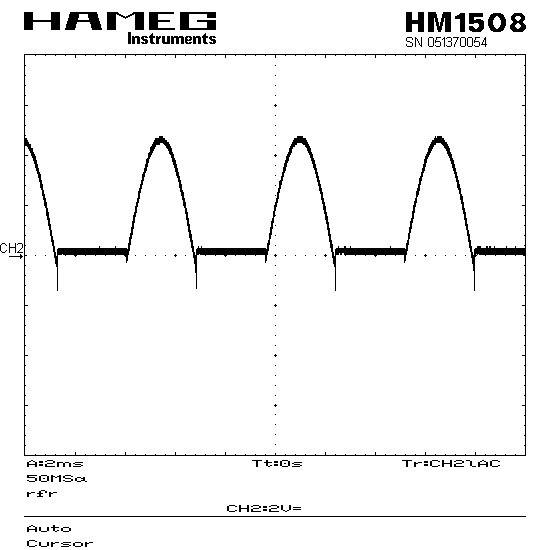
\includegraphics[scale=0.4]{SCR00018}}
				\subfigure[$ \Delta \phi = -90 ^\circ $]{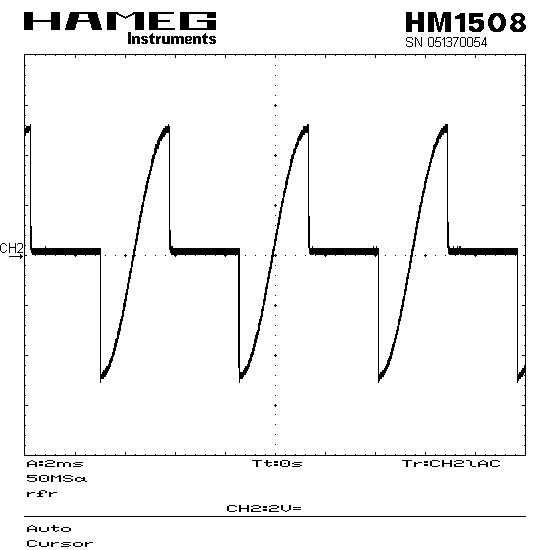
\includegraphics[scale=0.4]{SCR00019}}
			\end{figure}
			
			Im Prinzip kann man sich die Einwegegleichrichtung vorstellen wie eine Überlagerung/Multiplikation von einem Sinus mit einem Rechtecksignal, welches immer zwischen 0 (AUS) und 1 (AN) hin und her springt. Im linken Bild ist die Phasenverschiebung zwischen Sinus und Rechteck genau $ \Delta \phi = 0^\circ $ und im rechten Bild $ \Delta \phi =-90^\circ \simeq 270^\circ$.\\
			Die Zweiwegegleichrichtung ergibt die folgenden Bilder für $ \Delta \phi = 0^\circ $ und $ \Delta \phi = 270^\circ $:
			
			\begin{figure}[h!]
				\centering
				\subfigure[$Zweiwegegleichrichtung: \Delta \phi = 0^\circ $]{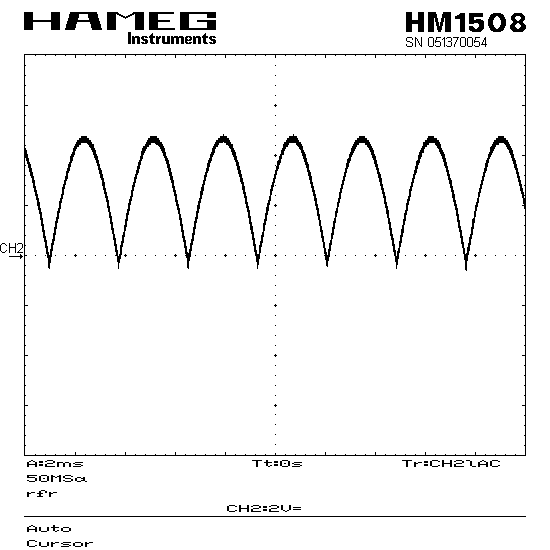
\includegraphics[scale=0.4]{SCR00020}}
				\subfigure[$ \Delta \phi = -90 ^\circ $]{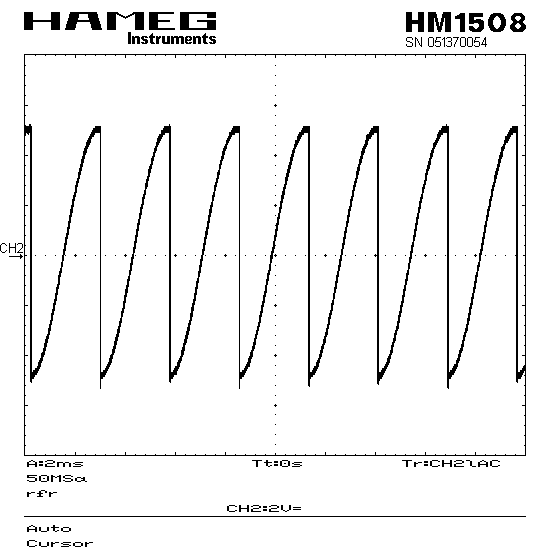
\includegraphics[scale=0.4]{SCR00021}}
			\end{figure}
			
			Anschießend untersuchten wir die Funktion des nachgeschalteten Tiefpasses. Diese wurde anhand der folgenden Bilder deutlich. Für die obigen Phasenverschiebungen und einen Tiefpass aus einem Widerstand mit $ R=18\ k\Omega $ und einem Kondensator mit $ C=10 \ \mu F $, haben wir Bilder aufgenommen. Nach Durchlauf durch den Kondensator ergaben sich für Zweiwegegleichrichtung folgende Verläufe.
			 \begin{figure}[h!]
			 	\subfigure[Signal nach Tiefpass:$\Delta \phi = 0^\circ $]{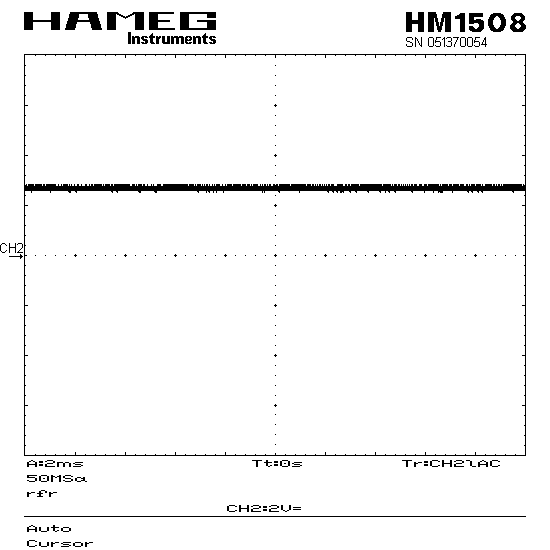
\includegraphics[scale=0.4]{SCR00022}}
			 	\subfigure[$ \Delta \phi = -90 ^\circ$]{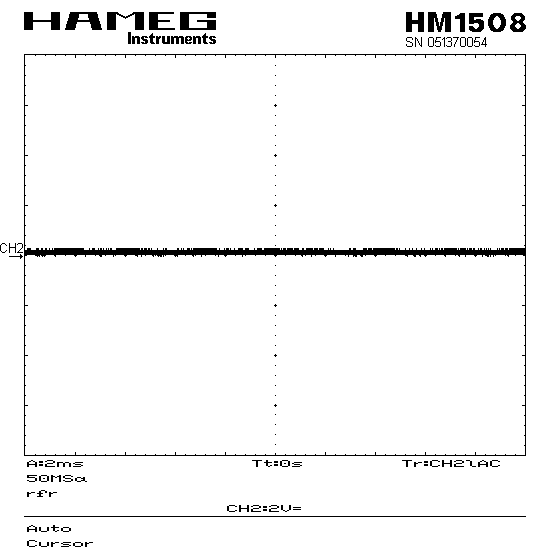
\includegraphics[scale=0.4]{SCR00023}}
			 \end{figure}
			 \newline
			 Ein Tiefpass mit hinreichend großer Zeitkonstante, hier $ \tau =RC=0,18 \ \Omega \cdot F $ erzeugt eine Gleichspannung, welche für $ \Delta \phi =0^\circ $ maximal, für $ \Delta \phi = \pm 90^\circ $ Null und für $ \Delta \phi =180^\circ $ minimal ist. Im Frequenzbereich wird Rauschen höherer Frequenzen durch den Tiefpass unterdrückt, sodass nach der Gleichrichtung nur noch das schmale Frequenzband um f=0 vorliegt.
			 \newline \\
			 In Versuchsteil 1.1.g sollte nun noch der Nachverstärker charakterisiert werden. Dazu nahmen wir eine Amplitudenübertragungsfunktion auf, woraus sich die Bandbreite bestimmen lässt. Da wir nur den rechten Zweig aufgenommen haben, lässt sich nur die obere Grenzfrequenz ablesen als $ f_{oben}=280\ kHz $. Als Bandbreite verwende ich nun einfach 2 mal die obere Grenzfrequenz, als ob der Graph symmetrisch zu f=0 Hz wäre. Diese Annahme ergibt eine Bandbreite von $ \Delta f =560\ Hz $.
			 \begin{figure}[h!]
				 \centering
				 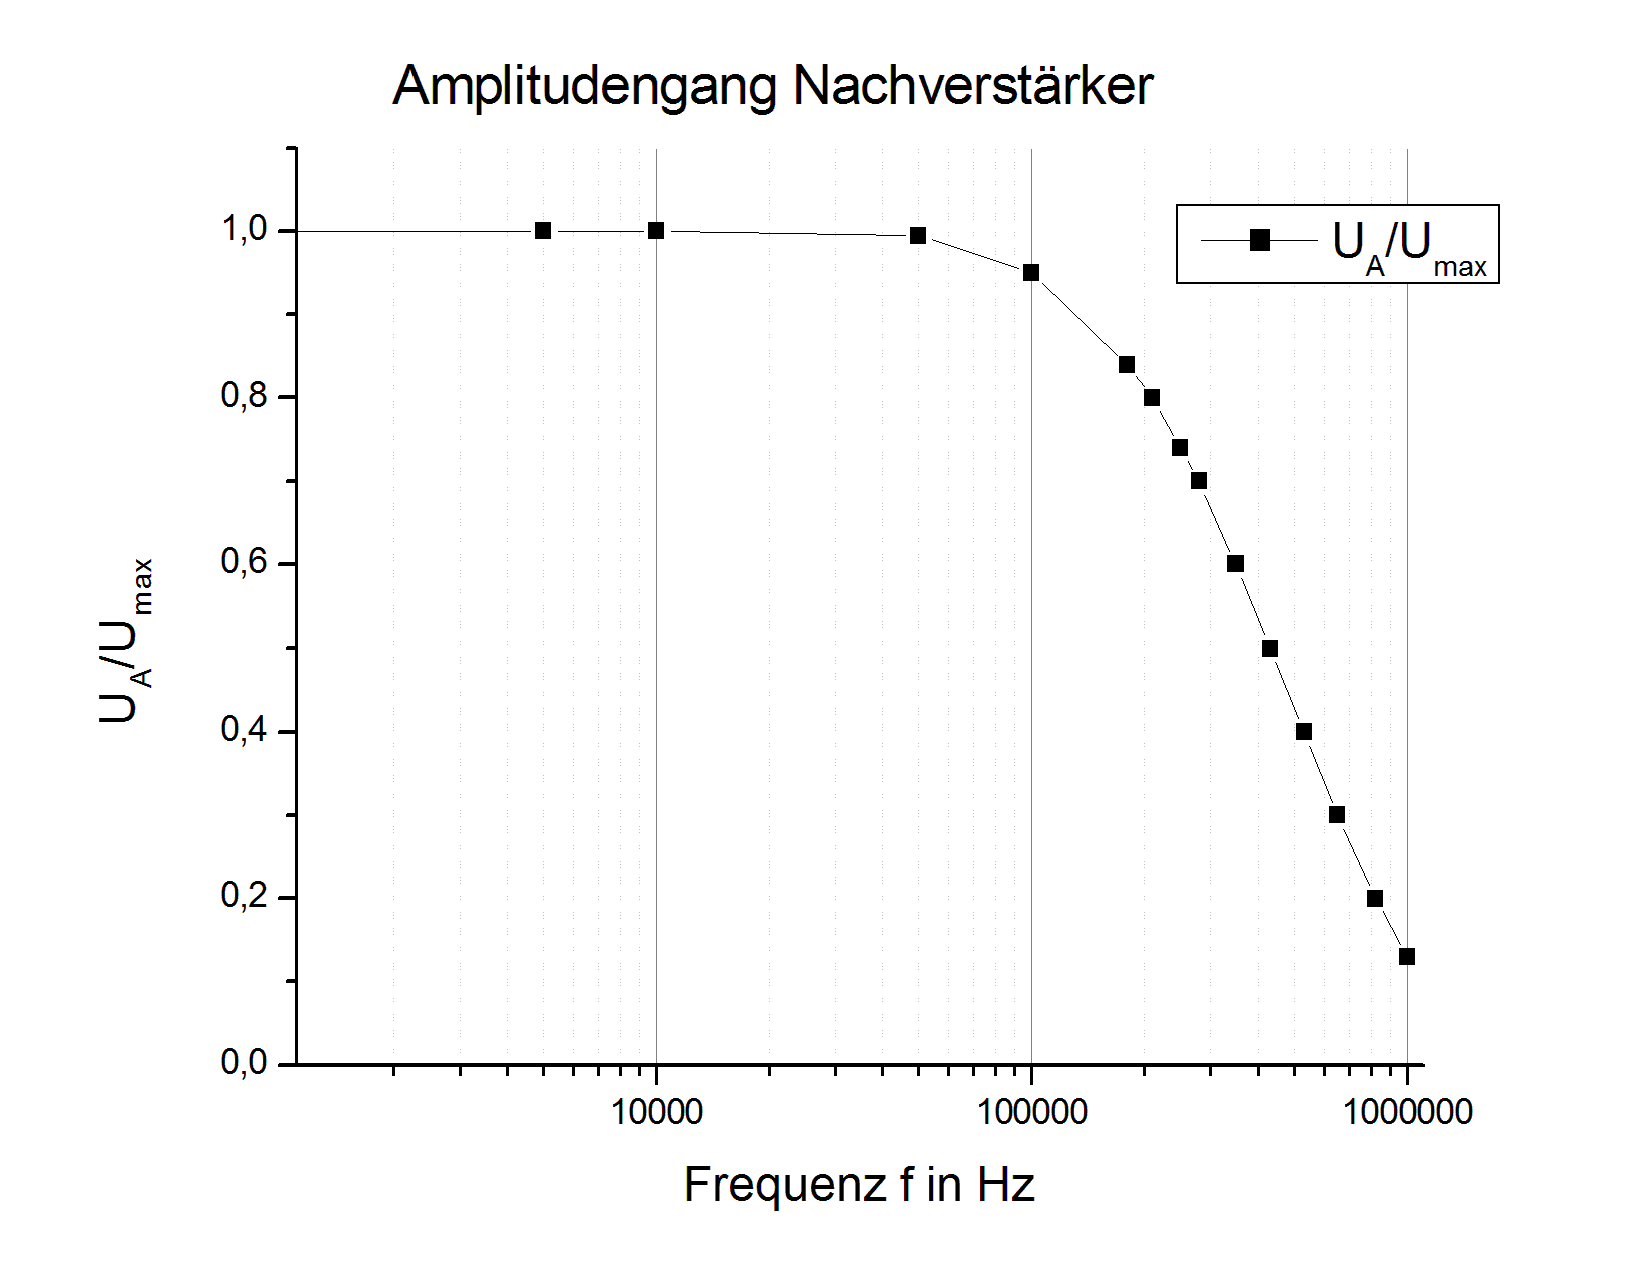
\includegraphics[scale=0.3]{A1g}
				 \caption{Amplitudengang Nachverstärker}
			 \end{figure}
			 
			 
	\clearpage

\section{Diskussion}
				
\end{document}